\section{Evidence Lower Bound}
Účelovou funkcí VAE je \emph{evidence lower bound}, dále jen ELBO (alternativně se lze setkat s pojmenováním \emph{variační dolní mez}).
Typicky je ELBO odvozena pomocí Jensenovy nerovnosti \cite[Sekce 4.2]{Wasserman2013}.
Autoři VAE \cite{Kingma2014} však využívají alternativního postup, jenž se chytře vyhýbá použití Jensenovy nerovnosti a nabízí větší míru \emph{tightness}
\footnote{Koncept z matematické teorie míry, který lze intuitivně popsat jako \emph{"sadu měr které příliš rychle  do nekonečna"}. \cite{Topsoee1974}}. 
Pro libovolnou konfiguraci inferenčního modelu $q_\phi(\textbf{z}\mid\textbf{x})$, včetně volby variačních parametrů $\phi$, dostáváme \cite[Rovnice 3]{Kingma2014}:

\begin{equation}
    \label{eq:vae_elbo}
    \mathcal{L}(\theta,\phi,x^{(i)}) = \mathds{E}_{q_\phi(z\mid x^{(i)})} \left[ \log p_\theta(x^{(i)}\mid z) \right] - \mathcal{D}_{KL}(q_\phi(z\mid x^{(i)})\parallel p_\theta(z))
\end{equation}

\autoref{eq:vae_elbo} je pro \textbf{variační autoenkodéry naprosto stěžejní} a slouží jako jádro pro jejich optimalizaci
\footnote{Historicky, matematický aparát \autoref{eq:vae_elbo} byl známý dlouho před formalizací VAE. Například Helmholtz Machines \cite{Dayan1995} využívají defacto identickou rovnici, ale s jedním zásadním rozdílem. Integrál v středních hodnotách VAE je v \cite[Rovnice 5]{Dayan1995} nahrazen sumou, jelikož Helmholtz Machines usuzují diskrétní rozdělení pravděpodobnosti pro latentní proměnné. A přesně tato volba znemožňuje transformaci, kterou VAE využívají k tomu, aby byl gradientní sestup ELBO efektivně řešitelný (tractable). \cite{Doersch2021}}. \cite{Doersch2021}

\begin{figure}[H]
    \centering
   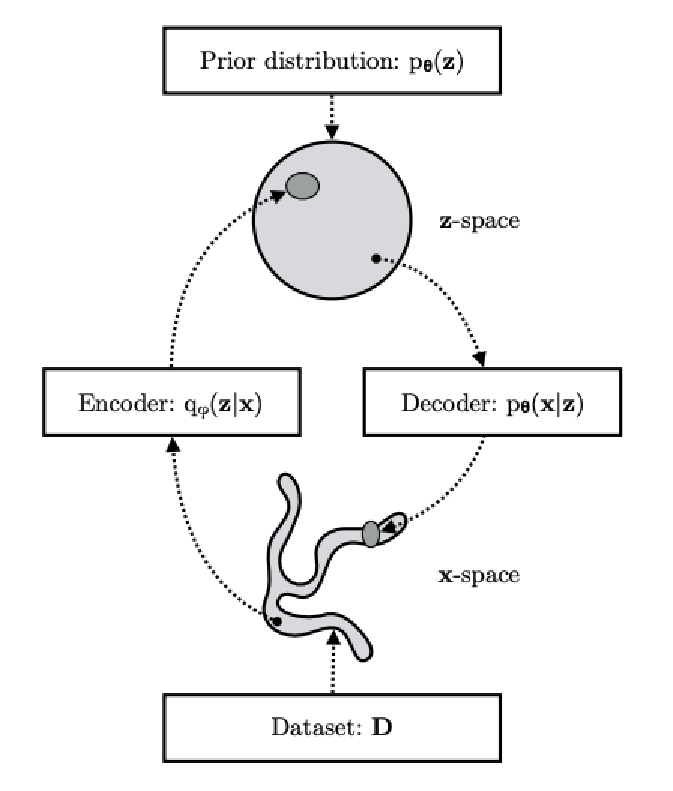
\includegraphics{figures/vae_schema.pdf}
   \caption{VAE se učí stochastické mapování mezi pozorovaným prostorem $x$, jehož empirické rozdělení pravděpodobnosti $q_\mathcal{D}(x)$ je typicky velmi komplikované, a latentním prostorem $z$, jehož rozdělení pravděpodobnosti je typicky relativně jednoduché (např. kulovité, jako na tomto obrázku). Generativní model se učí rozdělení pravděpodobnosti $p_\theta(x, z)$ (které lze faktorizovat jako $p_\theta(x, z) = p_\theta(z) p_\theta(x\mid z)$), s apriorním rozdělením skrze latentní prostor $p_\theta(z)$, a stochastický dekodér $p_\theta(x\mid z)$. Stochastický enkodér $q_\phi(z\mid x)$ aproximuje původní (ale efektivně neřešitelné) posteriorní rozdělení $p_\theta(z\mid x)$ generativního modelu. Obrázek včetně interpretace převzat z \cite{Kingma2019}.}
\end{figure}

\subsection{Odvození rovnice}
\begin{align}
    \log p_\theta(\textbf{x}) &= \mathds{E}_{q\phi(\textbf{z}\mid\textbf{x})}[\log p_\theta(\textbf{x})] \\
                              &= \mathds{E}_{q\phi(\textbf{z}\mid\textbf{x})} \left[ \log \left[ \frac{p_\theta(\textbf{x}, \textbf{z})}{p_\theta(\textbf{z}\mid\textbf{x})} \right] \right] \\
                              &= \mathds{E}_{q\phi(\textbf{z}\mid\textbf{x})} \left[ \log \left[ \frac{p_\theta(\textbf{x}, \textbf{z})}{q_\phi(\textbf{z}\mid\textbf{x})} \frac{q_\phi(\textbf{z}\mid\textbf{x})}{p_\theta(\textbf{z}\mid\textbf{x})} \right] \right] \\
                              &= \underbrace{ \mathds{E}_{q\phi(\textbf{z}\mid\textbf{x})} \left[ \log \left[ \frac{p_\theta(\textbf{x}, \textbf{z})}{q_\phi(\textbf{z}\mid\textbf{x})} \right] \right] }_\text{$ \iff \mathcal{L}_{\theta,\phi}(\textbf{x}) (ELBO)$} 
                              +  \underbrace{ \mathds{E}_{q\phi(\textbf{z}\mid\textbf{x})} \left[ \log \left[ \frac{q_\phi(\textbf{z}\mid\textbf{x})}{p_\theta(\textbf{z}\mid\textbf{x})} \right] \right] }_\text{$\iff D_{KL}(q_\phi(\textbf{z}\mid\textbf{x})\parallel p_\theta(\textbf{z}\mid\textbf{x}))$} \\ \label{eq:elbo_kl}
\end{align}

Druhý prvek \autoref{eq:elbo_kl} je Kullback-Lieblerova divergence (\autoref{sec:kl_divergence}) mezi $q_\phi(\textbf{z}\mid\textbf{x})$ (enkodérem) a $p_\theta(\textbf{z}\mid\textbf{x})$ (dekodérem), jejíž hodnota je \textbf{nezáporná}
\footnote{$\mathcal{D}_{KL}(q_\phi(\textbf{z}\mid\textbf{x})\parallel p_\theta(\textbf{z}\mid\textbf{x})) \geq 0$}.
Je-li hodnota této KL divergence nulová $\iff$ $q_\phi(\textbf{z}\mid\textbf{x})$ je rovno posteriorní distribuci původních dat (\emph{perfektně je rekonstruuje}). \cite{Kingma2019}


První prvek \autoref{eq:elbo_kl} je variační dolní mez (ELBO):

\begin{equation} \label{eq:elbo}
    \mathcal{L}_{\theta,\phi}(\textbf{x}) = \mathds{E}_{q\phi(\textbf{z}\mid\textbf{x})}[\log p_\theta(\textbf{x},\textbf{z}) - \log q_\phi(\textbf{z}\mid\textbf{x})]
\end{equation}

S ohledem na nenulovost KL divergence je tedy ELBO \textbf{dolní mezí}\footnote{Od tud \emph{evidence \textbf{lower bound}}} log-likelihood původních dat. \cite{Kingma2014}, \cite{Goodfellow2016}
Dle \autoref{eq:elbo} platí:

\begin{align}
    \mathcal{L}_{\theta,\phi}(\textbf{x}) &= \log p_\theta(\textbf{x}) - D_{KL}(q_\phi(\textbf{z}\mid\textbf{x})\parallel p_\theta(\textbf{z}\mid\textbf{x})) \\ \label{eq:vae_optimization_objective}
                                          &\leq \log p_\theta(\textbf{x})
\end{align}

V tomto případě tedy pozoruhodně tato KL divergence určuje hned dvě \emph{vzdálenosti} \cite{Kingma2019}:
\begin{enumerate}
    \item KL divergenci aproximace posteriorního rozdělení od původního posteriorního rozdělení (z definice KL divergence)
    \item \emph{Mezeru} mezi ELBO $\mathcal{L}_{\theta,\phi}(\textbf{x})$ a \emph{marginal likelihood} $\log p_\theta(\textbf{x})$. Tuto \emph{mezeru} také nazýváme mírou \emph{tightness} této meze ($\implies$ vyhnutí se použití Jensenově nerovnosti). Čím lépe $q_\phi(\textbf{z}\mid\textbf{x})$ aproximuje $p_\theta(\textbf{z}\mid\textbf{x})$, s ohledem na KL divergenci, tím menší tato \emph{mezera} je.
\end{enumerate}

\subsection{Optimalizační cíle}
Z \autoref{eq:vae_elbo} plynou důsledky maximalizace ELBO $\mathcal{L_{\theta,\phi}}$ s ohledem na parametry $\boldsymbol{\theta}$ a $\boldsymbol{\phi}$.
A to sice současná optimalizace dvou kritérií, která jsou pro výkonnost VAE stěžejní \cite{Kingma2019}:

\begin{enumerate}
    \item \emph{Přibližná} maximalizace marginální věrohodnosti $p_\theta(\textbf{x})$, což implikuje \emph{zlepšení} generativního modelu \footnote{Tedy \emph{věrohodnosti} rekonstrukce původních dat}.
    \item Minimalizace KL divergence aproximace mezi $q_\phi(\textbf{z}\mid\textbf{x})$ a původní posteriorní distribucí $p_\theta(\textbf{z}\mid\textbf{x})$. Tedy $q_\phi(\textbf{z}\mid\textbf{x})$ (enkodér) se \emph{zlepší}.
\end{enumerate}